\documentclass{beamer}
\mode<presentation>
\usetheme{CambridgeUS}
\usepackage[russian]{babel}
\usepackage[utf8]{inputenc}
\usepackage[T2A]{fontenc}
\usepackage{sansmathaccent}
\pdfmapfile{+sansmathaccent.map}
\title{Модуляция, фазовые преобразования и другие эффекты}
\author{Наумов Д.А.}
\date[16.04.2014] {Компьютерные музыкальные технологии и звуковой дизайн, 2014}

\begin{document}

%ТИТУЛЬНЫЙ СЛАЙД
\begin{frame}
  \titlepage
\end{frame}

%СОДЕРЖАНИЕ ЛЕКЦИИ
\begin{frame}
  \frametitle{Содержание лекции}
  \tableofcontents
\end{frame}

%РАЗДЕЛ 1
\section{Эффекты модуляции}
\subsection{Основные понятия}
\begin{frame}
  \textbf{Модуляция} (лат. \textit{modulatio}~--- размеренность, ритмичность)~--- процесс изменения одного или нескольких параметров высокочастотного несущего колебания по закону низкочастотного информационного сигнала (сообщения).

  ~

  \begin{block}{Виды модуляции}
    \centering{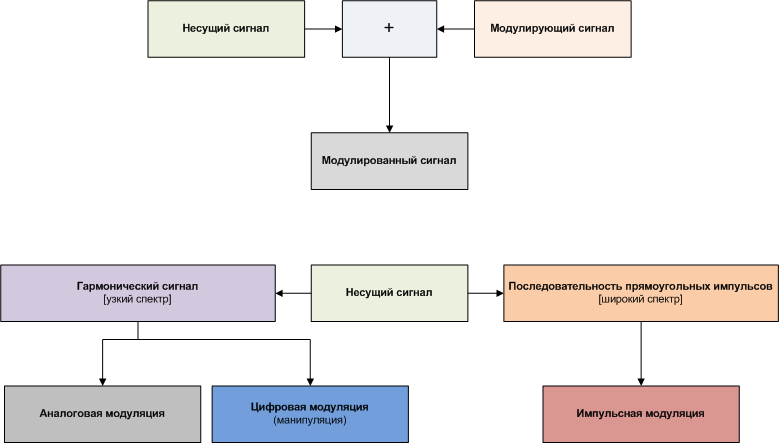
\includegraphics[width=0.75\textwidth]{pic-modulation-01}}
  \end{block}
\end{frame}

\begin{frame}
  В качестве несущего могут быть использованы колебания различной формы (прямоугольные, треугольные и т. д.), однако чаще всего применяются гармонические колебания.

  ~

  \begin{block}{Периодические сигналы различной формы}
    \centering{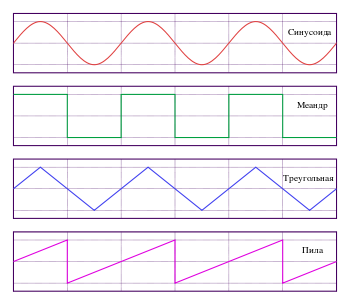
\includegraphics[width=0.5\textwidth]{pic-modulation-02}}
  \end{block}
\end{frame}

\begin{frame}
  \begin{block}{Периодические сигналы различной формы}
    \begin{itemize}
      \item \textit{Синусоида}. Амплитуда сигнала соответствует тригонометрической функции синуса $sin(x)$, изменяющейся по времени.
      \item \textit{Меандр}. Этот сигнал, как правило, используется для представления и передачи цифровых данных. Прямоугольные импульсы с постоянным периодом содержат нечётные гармоники, которые попадают на -6~дБ/октаву.
      \item \textit{Треугольная волна}. Включает в себя нечётные гармоники, которые попадают на -12~дБ/октаву.
      \item \textit{Пилообразная волна}. Выглядит как зубья пилы. Используется в качестве отправной точки субтрактивного синтеза, так как пилообразная волна с постоянным периодом содержит чётные и нечётные гармоники, которые попадают на -6~дБ/октаву.
    \end{itemize}
  \end{block}
\end{frame}

\subsection{Амплитудное вибрато}
\begin{frame}
\textbf{Амплитудное вибрато} (англ. \emph{amplitude modulation})~--- звуковой эффект или соответствующее устройство, реализующее периодическое изменение уровня громкости (амплитуды сигнала), характеризуется пульсирующим звучанием.

~

При быстром изменении амплитуды от 100\% до 0\% можно добиться эффекта тремоло.

~

\textbf{Тремоло} (итал. \emph{tremolo}, букв.~--- дрожащий)~--- приём игры на струнных, клавишных, ударных и других музыкальных инструментах: многократное быстрое повторение одного звука либо быстрое чередование двух несоседних звуков, двух созвучий (интервалов, аккордов), отдельного звука и созвучия.
\end{frame}

\begin{frame}
  В пакете \emph{Waves} плагин \emph{MondoMod} представляет собой эффект, включающий \emph{амплитудную модуляцию} (тремоло), \emph{частотную модуляцию} (вибрато) и \emph{фазовую модуляцию}.

  ~

  \begin{block}{Окно эффекта \emph{Waves MondoMod}}
    \centering{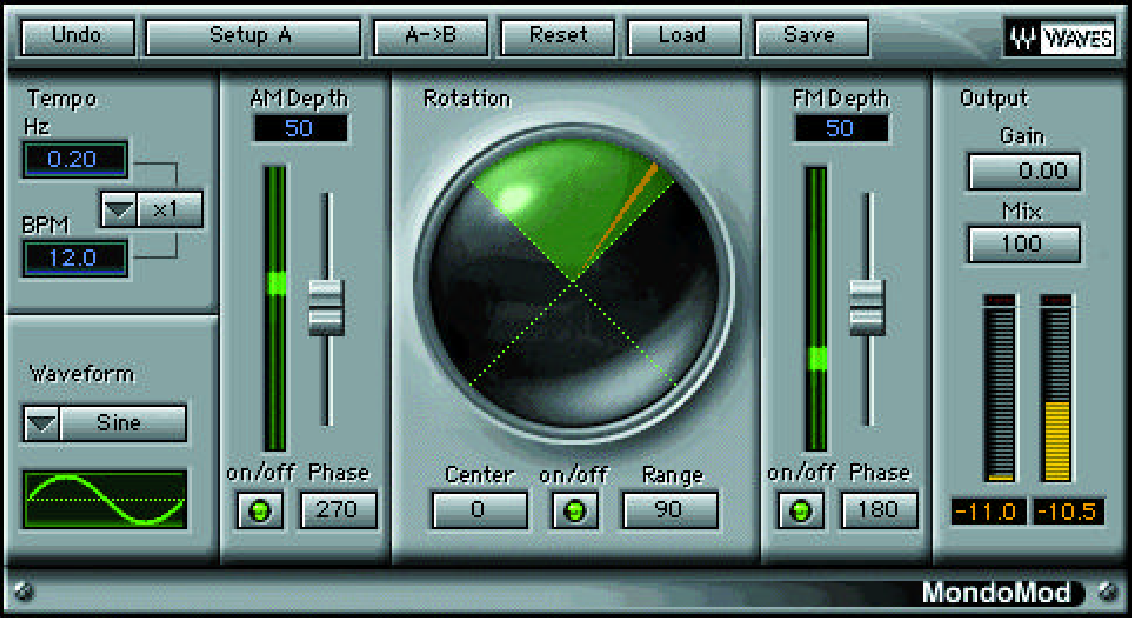
\includegraphics[width=0.75\textwidth]{pic-mondomod-01}}
  \end{block}
\end{frame}

\subsection{Эффект хоруса}
\begin{frame}
  \textbf{Хорус} (англ. \textit{chorus})~--- звуковой эффект или соответствующее устройство, которое имитирует хоровое звучание музыкальных инструментов.

  ~

  Эффект реализуется следующим образом:
  \begin{enumerate}
    \item Входной сигнал разделяется на два независимых сигнала, один из которых остаётся без изменений, в то время как другой поступает на линию задержки.
    \item В линии задержки осуществляется задержка сигнала на 20-30 мс, причём время задержки изменяется в соответствии с сигналом генератора низких частот.
    \item На выходе задержанный сигнал смешивается с исходным.
  \end{enumerate}
  
  ~
  
  \emph{Генератор низких частот} осуществляет модуляцию времени задержки сигнала: он вырабатывает колебания определённой формы, лежащие в пределах от 3 Гц и ниже. Изменяя частоту, форму и амплитуду колебаний низкочастотного генератора, можно получать различный выходной сигнал.
\end{frame}

\begin{frame}
  Эффект имеет следующие параметры:
  \begin{itemize}
    \item \textbf{Глубина} (\textit{depth})~--- характеризует диапазон изменения времени задержки.
    \item \textbf{Скорость} (\textit{speed}, \textit{rate})~--- быстрота изменения "<плавания"> звука, регулируется частотой низкочастотного генератора.
    \item \textbf{Форма волны генератора низкой частоты} (\textit{LFO waveform}).
    \item \textbf{Баланс} (\textit{balance}, \textit{mix}, \textit{dry/wet})~--- соотношение необработанного и обработанного сигналов.
  \end{itemize}
\end{frame}

\begin{frame}
  В \emph{Adobe Audition} команда \textit{Effects > Modulation > Chorus} открывает диалоговое окно эффекта хора.

  ~

  \begin{block}{Окно эффекта хорус}
    \centering{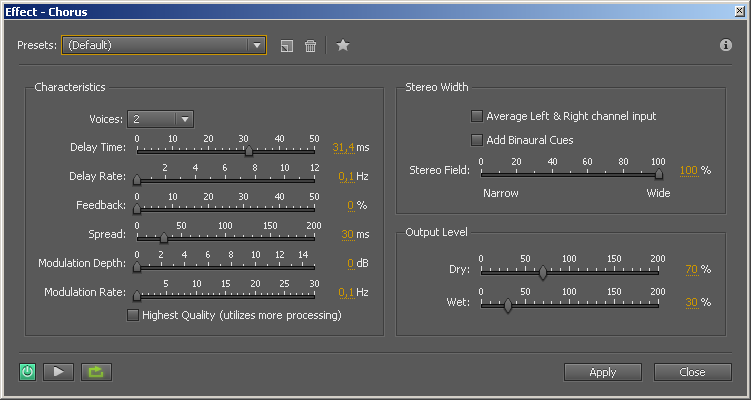
\includegraphics[width=0.75\textwidth]{pic-auchorus-01}}
  \end{block}
\end{frame}

\subsection{Эффект фланжер}
\begin{frame}
  \textbf{Фланжер} (англ. \textit{flange}~--- фланец, гребень, бобина)~--- звуковой эффект или соответствующее устройство. По принципу работы напоминает хорус и отличается от него временем задержки (5—15 мс) и наличием обратной связи.

  ~
    
  Фланжер напоминает взлёт самолёта и данный эффект он был популярен в 1960-х, когда музыканты активно применяли его для создания психоделического звучания.
  
  ~
  
  В результате применения эффекта частотная характеристика представляет ряд максимумов и минимумов, напоминая гребень, откуда и происходит название. Фаза сигнала обратной связи иногда инвертируется, тем самым достигается дополнительная вариация звукового сигнала.
\end{frame}

\begin{frame}
  В \emph{Adobe Audition} диалоговое окно эффекта \textit{Flanger} открывается командой \textit{Effects > Modulation > Flanger}.

  ~

  \begin{block}{Окно эффекта фланжер}
    \centering{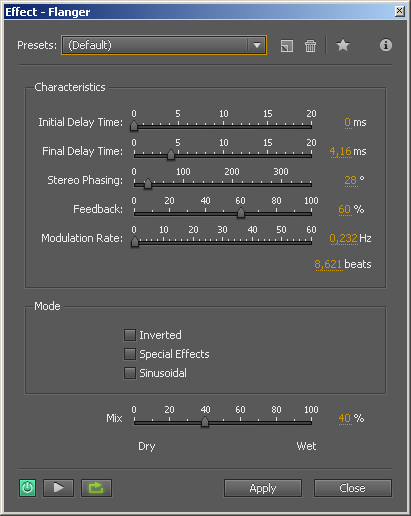
\includegraphics[width=0.75\textwidth]{pic-auflanger-01}}
  \end{block}
\end{frame}

\begin{frame}
  Эффект \emph{MetaFlanger}, входящий в пакет \emph{Waves}, может быть использован для создания различных эффектов: фланжера, фейзера, хоруса и других эффектов, построенных на основе модуляции.

  ~

  \begin{block}{Окно эффекта \emph{MetaFlanger}}
    \centering{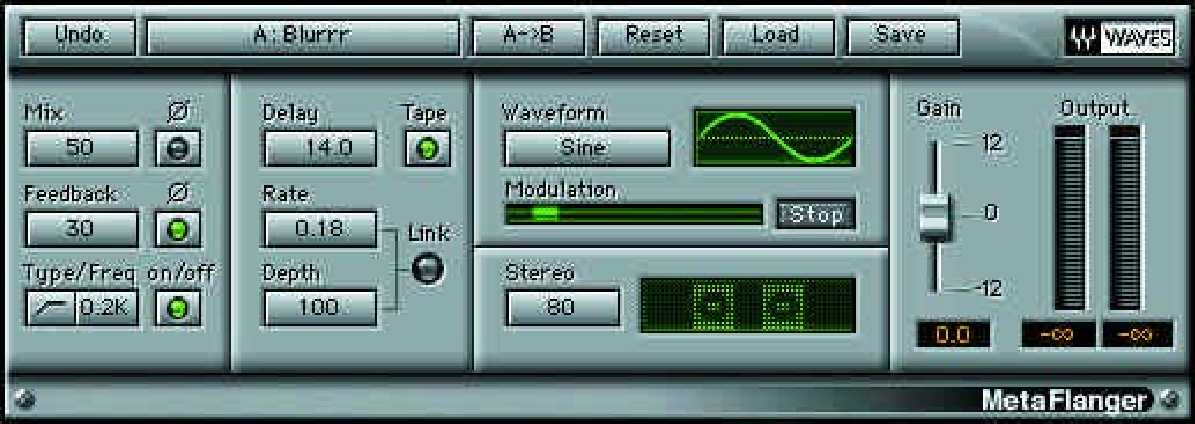
\includegraphics[width=0.75\textwidth]{pic-metaflanger-01}}
  \end{block}
\end{frame}

\subsection{Эффект фейзер}
\begin{frame}
  \textbf{Фэйзер} (англ. \textit{phaser}), также часто называемый фазовым вибрато~--- звуковой эффект, который достигается фильтрацией звукового сигнала с созданием серии максимумов и минимумов в его спектре. Положение этих максимумов и минимумов варьируется на протяжении звучания, что создает специфический круговой (англ. \textit{sweeping}) эффект.

  \begin{block}{Результат применения фейзера}
    \centering{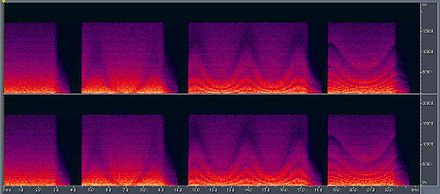
\includegraphics[width=0.75\textwidth]{pic-phaser-03}}
  \end{block}
\end{frame}

\begin{frame}
  \begin{block}{Спектрограмма сигнала, пропущенного через 8-каскадный фильтр без обратной связи, отношение обработанного и необработанного сигнала: 50/50}
    \centering{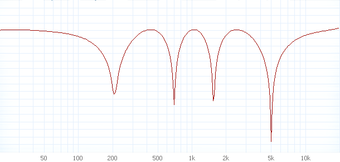
\includegraphics[width=0.75\textwidth]{pic-phaser-01}}
  \end{block}
\end{frame}

\begin{frame}
  \begin{block}{Спектрограмма сигнала, пропущенного через 8-каскадный фильтр с 50\% обратной связью, отношение обработанного и необработанного сигнала: 50/50}
    \centering{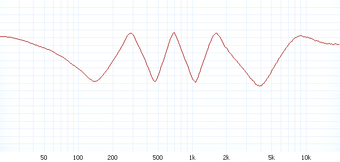
\includegraphics[width=0.75\textwidth]{pic-phaser-02}}
  \end{block}
\end{frame}

\begin{frame}
  В \textit{Adobe Audition} эффект реализован следующим образом: имеется группа фильтров, которые сдвигают фазу сигнала до и после частоты среза. При применении эффекта фильтры периодически переключаются.

  \begin{block}{Окно эффекта фейзера}
    \centering{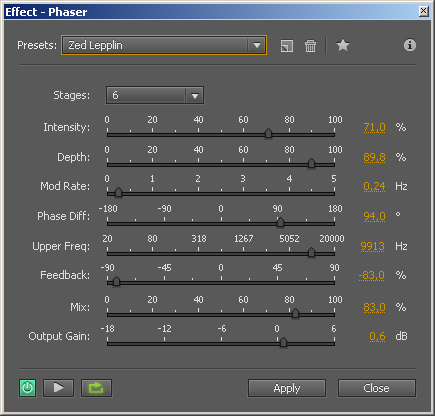
\includegraphics[width=0.5\textwidth]{pic-auphaser-01}}
  \end{block}
\end{frame}

\begin{frame}
  Эффект \emph{Enigma}, входящий в пакет \emph{Waves}, можно описать как сложный фэйзер/фланжер с реверберацией и обратной связью со сложной фильтрацией, а также дополнительной модуляцией.

  \begin{block}{Окно эффекта \emph{Waves Enigma}}
    \centering{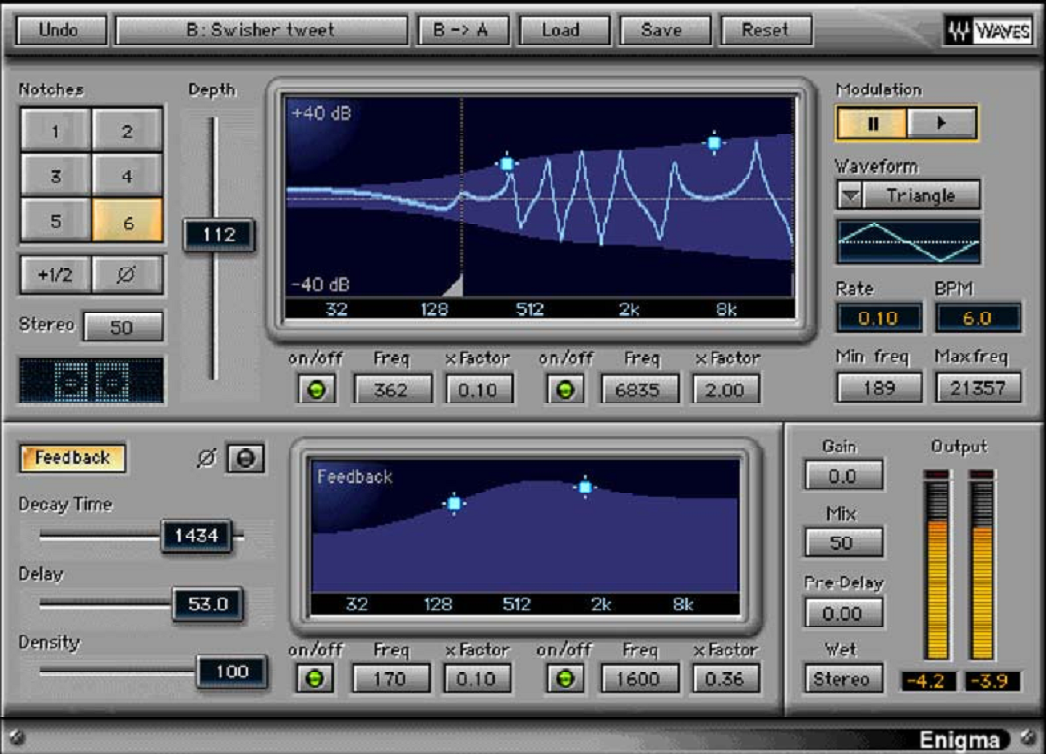
\includegraphics[width=0.75\textwidth]{pic-enigma-01}}
  \end{block}
\end{frame}

\section{Фазовые преобразования}
\begin{frame}
  В программах цифровой обработки звука есть несколько средств, предназначенных для изменения стерео образа звука:
  \begin{itemize}
    \item преобразования моно в стерео и обратно,
    \item расширения стерео-панорамы,
    \item имитации вращения стереополя вокруг слушателя и т.д.
  \end{itemize}

  ~

  В \textit{Adobe Audition} к эффектам подобного назначения относятся:
  \begin{itemize}
    \item \textit{Center Channel Extractor}~--- извлечение/удаление центрального канала;
    \item \textit{Graphic Phase Shifter}~--- инструмент для изменения фаз частотных составляющих сигнала.
  \end{itemize}
\end{frame}

\begin{frame}
  Команда меню \textit{Effects > Stereo Imagery > Center Channel Extractor} вызывает диалоговое окно эффекта, который позволяет сохранять или удалять совпадающие частоты левого и правого каналов (т.е звуков, которые панорамированы в центр: голос, бас и партии главных инструменты).

  \begin{block}{Окно эффекта \emph{Center Channel Extractor}}
    \centering{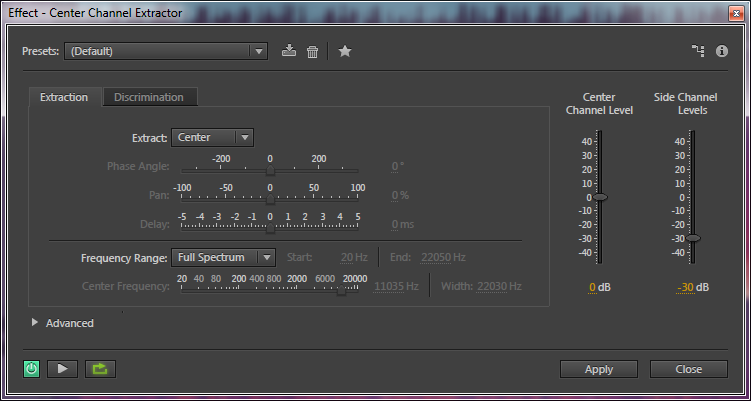
\includegraphics[width=0.75\textwidth]{pic-aucenterchannel-01}}
  \end{block}
\end{frame}

\begin{frame}
  Команда меню \textit{Effects > Stereo Imagery > Graphic Phase Shifter} вызывает диалоговое окно эффекта, позволяющего вручную задать график зависимости изменения фазы спектральных составляющих сигнала в зависимости от частоты.
.

  \begin{block}{Окно эффекта \emph{Graphic Phase Shifter}}
    \centering{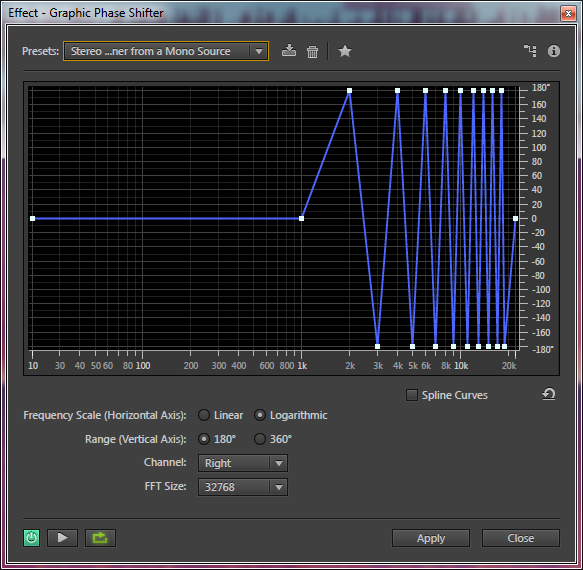
\includegraphics[width=0.5\textwidth]{pic-auphaseshift-01}}
  \end{block}
\end{frame}

\section{Другие эффекты}
\begin{frame}
  \textbf{Питч-шифтер} (англ. \textit{pitch shifter})~--- звуковой эффект или соответствующее устройство, добавляющее к сигналу его копию, отстоящую от основного тона на любой интервал в пределах двух октав вверх или вниз.

  В \emph{Adobe Audition} инструмент \textit{Time And Pitch > Stretch and Pitch} позволяет изменять высоту звука, темп или оба данных параметров одновременно. Данный эффект можно использовать для транспонирования песни (не изменяя темп композиции), или для изменения скорости без изменения высоты тона.

  \begin{block}{Окно эффекта \emph{Stretch and Pitch}}
    \centering{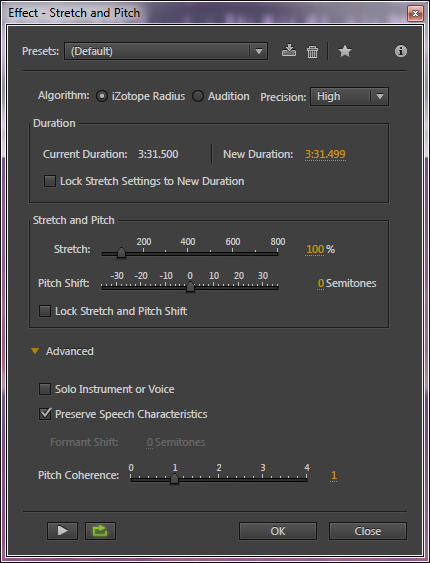
\includegraphics[width=0.5\textwidth]{pic-austretch-01}}
  \end{block}
\end{frame}

\begin{frame}
  В \emph{Adobe Audition} при выполнении команды \textit{Time And Pitch > Manual Pitch Correction} редактор переходит в режим \emph{Spectral Pitch Display} и появляется окно, в котором можно выбрать канал и режим сглаживания огибающей. Сам же эффект позволяет при помощи огибающей задать график изменения высоты тона звука в зависимости от времени.

  \begin{block}{Окно эффекта \emph{Manual Pitch Correction}}
    \centering{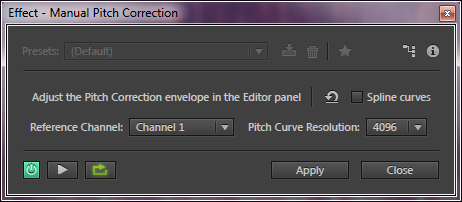
\includegraphics[width=0.5\textwidth]{pic-aupitch-02}}
  \end{block}
\end{frame}

\begin{frame}
  \begin{block}{Режим \emph{Spectral Pitch Display}}
    \centering{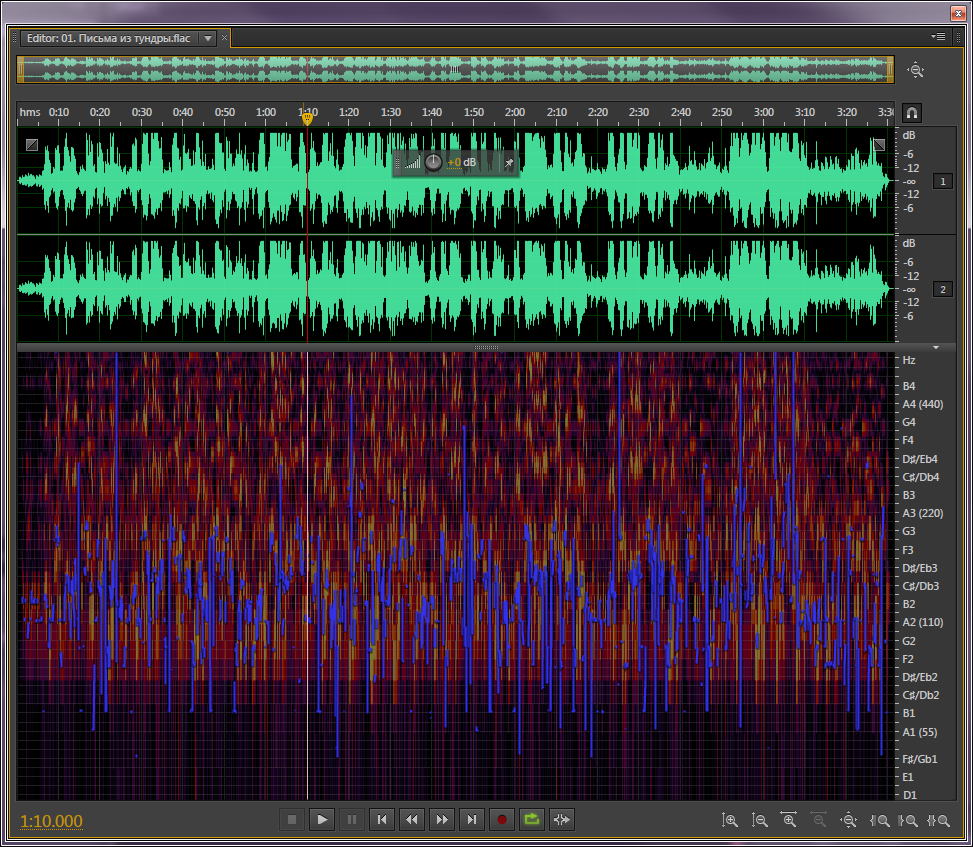
\includegraphics[width=0.75\textwidth]{pic-aupitch-01}}
  \end{block}
\end{frame}

\begin{frame}
  \textbf{Дисторшн} (англ. \textit{distortion}~---искажение)~--- звуковой эффект, достигаемый искажением сигнала путём его "<жёсткого"> ограничения по амплитуде, или устройство, обеспечивающее такой эффект. Наиболее часто применяется в музыкальных жанрах хард-рок, метал и панк-рок в сочетании с электрогитарой, а также в хардкор-техно и особенно в спидкоре и брейккоре с драм-машиной. 
  
  ~
  
  Иногда этим термином обозначают группу однотипных звуковых эффектов (овердрайв, фузз и прочие), реализующих нелинейное искажение сигнала. Их также называют эффектами "<перегруза">, а соответствующие устройства~--- "<искажателями">.

  ~
 
  \textbf{Овердрайв} (англ. \textit{overdrive} или \textit{перегруз})~--- звуковой эффект, достигаемый искажением сигнала путём его "<мягкого"> ограничения по амплитуде, или соответствующее устройство.
 \end{frame}

\begin{frame}
  \begin{block}{Пример сигналограммы с эффектами дисторшн и овердрайв}
    \centering{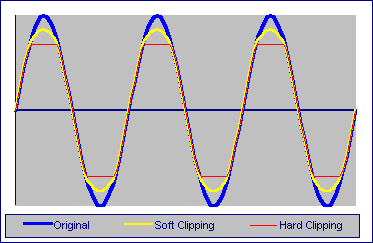
\includegraphics[width=0.75\textwidth]{pic-overdrive-01}}
  \end{block}
\end{frame}

\begin{frame}
  Эффект повторного звучания может быть вызван распространением звука от источника к приемнику различными путями: звук может приходить напрямую и может отразиться от препятствия, находящегося чуть в стороне от прямого пути).

  ~
  
 При этом время задержки остается постоянным. В реальной жизни этому соответствует ситуация, когда источник звука, приемник звука и отражающие предметы неподвижны друг относительно друга, при этом частота звука не изменяется.

 ~
 
 Если же какой-либо из трех элементов подвижен, то частота принимаемого звука изменяется~--- это проявление \textbf{эффекта Доплера}, который в школьных учебниках традиционно поясняется на примере изменения высоты звучания гудка движущегося паровоза.
\end{frame}

\begin{frame}
  Для вызова эффекта в \emph{Adobe Audition} необходимо выполнить команду \textit{Effects > Special > Doppler Shifter}.
  
  ~  
  
  \begin{block}{Окно эффекта \emph{Doppler Shifter}}
    \centering{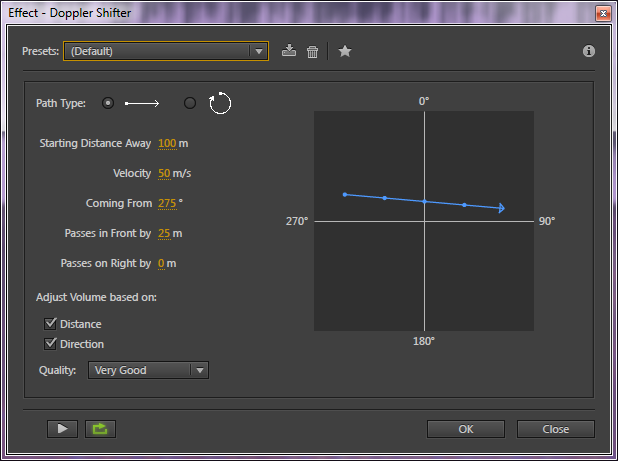
\includegraphics[width=0.65\textwidth]{pic-audoppler-01}}
  \end{block}
\end{frame}

\section{Примеры применения некоторых эффектов}
\begin{frame}
  \begin{block}{Хорус}
     Часть 1 демонстрирует применение эффекта для обработки речи. Вы можете слышать исходный голос в середине с двумя фантомными голосами с немного другой высотой тона по бокам. 

     ~

     Часть 2 является тем же звуком с монофоническим эффектом. Она звучит в чем-то похоже на эхо, но в ней есть те же вариации высоты тона. 

~

     Часть 3~--- это запись музыки с эффектом Chorus (часто используется для усиления вокала солиста). 

~

     В части 4 использована более длинная задержка, чтобы нереалистично расширить изменение высоты тона фантомных голосов.

    Часть 5. Первый звук является вертолетом без обработки эффектом. Второй звук является тем же звуковым эффектом, обработанным хорусом.
  \end{block}  
\end{frame}
\begin{frame}
  \begin{block}{Фланжер}
     Часть 1 является необработанными образцами голоса и музыки, приведенными для сравнения.

~

Чтобы добавить вибрато в голос (часть 2), установите задержку в 2мсек, скорость в 6,5 Гц, величину обратной связи в 5 процентов, а микс в 100 в процентов.

~

Для классического эффекта полета (wooshing) для музыки или звуковых эффектов (часть 3) используйте глубокую обратную связь. Установите задержку в 0 мсек, скорость в 0,15 Гц, глубину в 10 процентов, микс в 50 процентов и обратную связь в 90 процентов. Попробуйте также обратную связь, равную -90 процентам.
  \end{block}  
\end{frame}

\begin{frame}
  \begin{block}{Фланжер}
Более тонкий эффект полета без обратной связи может добавить движение в звуковые эффекты. Часть 4 трека является постоянным звуком вертолета в наружной обстановке, без обработки. Но с некоторым добавлением фленджера (часть 5), вы можете заставить вертолет двигаться. Для этого были установлены 0 мсек задержки, 0,1 Гц скорости, 10 процентов глубины, 50 процентов микса и не было обратной связи.

~

Чтобы поместить голоса под воду (часть 6), используйте 4 мсек задержки, 1,5 Гц скорости, 15 процентов глубины, 100 процентов микса без обратной связи.  
  \end{block}  
\end{frame}

\end{document}
